\documentclass{article}

\usepackage{fullpage}
\usepackage[english]{babel}
\usepackage[utf8x]{inputenc}
\usepackage{amsmath}
\usepackage{amssymb}
\usepackage{graphicx}
\usepackage[colorinlistoftodos]{todonotes}
%\usepackage[]{algorithm2e}
\usepackage[linesnumbered]{algorithm2e}
\usepackage{enumerate,url}
\usepackage{hyperref}
\hypersetup{colorlinks=true}
\usepackage{enumitem}

\title{CSE-6140/CX-4140 Algorithm Problems\\by\\Shahrokh Shahi }
\author{}
\date{}
\begin{document}
\maketitle

\noindent\fbox{\parbox{\dimexpr\textwidth-2\fboxsep-2\fboxrule\relax}{
\vspace{2mm}
Please upload two files: 
\begin{enumerate}
 \item A single PDF named \texttt{assignment.pdf} containing your solutions.
 \item 
\end{enumerate}
}}
\section*{ASSIGNMENT PROBLEMS}
\section{Dynamic Programming: Atlanta MARTA [xx pts]}
The  Metropolitan  Atlanta  Rapid Transit  Authority  (MARTA) is  the  principal  public  transportoperator in the Atlanta metropolitan area. It was Formed in 1971 as strictly a bus system, and today, it is transporting almost 450,000 passengers a day (bus and train). Currently, MARTA Passes are the cheapest option for those who regularly use MARTA for transportation. Assume the MARTA Passes are sold in three following forms:

\begin{itemize}
\item Daily: A 1-day pass sold for $tickets[0]$ dollars;
\item Weekly: A 7-day pass sold for $tickets[1]$ dollars;
\item Monthly: A 30-day pass sold for $tickets[2]$ dollars.
\end{itemize}

For instance, $tickets = {2, 7, 20}$ means we need to pay $\$2$, $\$7$, and $\$20$ for each daily, weekly,and monthly pass, respectively. The passes allow consecutive days of travel.  For example, if we get a weekly pass on day 5, then we can travel for 7 consecutive days which are: day 5, 6, 7, 8, 9,10, and 11. George P. Burdell is a student at Georgia Tech and he has already organized his commuting plan for  the  upcoming  year.  In  his  plan,  each   day of  year  is  specified   by an  integer   identification number from 1 to 365. Therefore, he can represent his commuting plan as an array of integers. For instance, days = {8, 9, 10, 11, 14, 17, 18, ...} means George needs to commute to the school on the 8th, 9th, 10th, 11th, ... days of year. He asked you to help him find the minimum amount of money that he should spend to purchase MARTA Passes for commuting to school in the next year. 

\begin{itemize}
\item[a)] (3 pts) Prove the optimal substructure.
\item[b)] (4 pts) Write a recursive expression for calculating min Cost including the base case.
\item[c)] (6 pts) Give the pseudocode of  a   linear   Dynamic   Programming   algorithm   to   return   the   minimum   cost   of commuting  every day in the array “days”, if the cost of MARTA passes is given in a three-element array “tickets”.	Analyze the space and time complexity of your algorithm.
\end{itemize}
%\clearpage
% -----------------------------------------------------------------------
\color{blue}
\subsection*{Solution}

\subsubsection*{Optimal Substructure}

We are given an array of integer numbers representing the days that George wants to commute to school. $days = \{d_1, d_2, \ldots, d_n \}$, and a three-element array $tickets = \{t_1, t_2, t_3\}$. we want to calculate the minimum possible value that George has to pay for buying MARTA passes. Let $OPT[i]$ denotes the minimum amount of money George needs to pay to fulfill the plan from day $i$ to the end of the plan. Therefore, the minimum cost of commuting for the entire plan is $OPT[1]$.
There can be two approaches to solve this problem: \\
\begin{itemize}
\item\textit{Approach 1: Iterate over all days}\\
Starting from day one, if George doesn't want to travel today, there is no need to buy a MARTA pass today. Therefore, it is strictly better to wait until the day that he needs to travel, say day $i$. Then, he will have three options: buying a 1-day, 7-day, or 30-day MARTA pass:
\begin{itemize}
	\item If he buys a 1-day pass: he needs to pay $tickets[0]$ dollars and the next subproblem is $OPT[i+1]$ because the 1-day pass is only valid for one day and for the next day he has to pay $OPT[i+1]$ dollars for commuting from day $i+1$ to the end of the plan.
	\item If he buys a 7-day pass: he needs to pay $tickets[1]$ dollars and the next subproblem is $OPT[i+7]$ since the 7-day pass is valid for 7 days (from the day of purchase), and thus after that 7 days, he has to pay $OPT[i+7]$ dollars for commuting from day $i+7$ to the end of the plan.
	\item Similarly, if he buys a 30-day pass: he needs to pay $tickets[2]$ dollars and the next subproblem is $OPT[i+30]$
\end{itemize}

Therefore, if George needs to travel in day $i$, the optimum amount of money can be obtained by taking the minimum values of these three:
$$
OPT[i] = \min\{ tickets[0] + OPT[i+1], tickets[1] + OPT[i+7] ,  tickets[2] + OPT[i+30]\}
$$


The solution of these three subproblems, $OPT[i+1]$, $OPT[i+7]$, and $OPT[i+30]$ are minimum. For the sake of contradiction, assume these three values are not the minimum solutions. Therefor, there must exist other optimum solutions with the less ticket cost. Then, we can substitute the solution(s) of subproblem(s) with these minimum values. That implies we obtain less value for $OPT[i]$, the cost of tickets for the commuting plan from day $i$ which is a contradiction because we started with this assumption that $OPT[i]$ is the minimum ticket cost. Thus, this problem has optimal substructures. $\blacksquare$

%But we can only consider the days that their identification number is in the commuting plan. 

\item\textit{Approach 2: Iterate over the days of the commuting plan}\\
In the first approach, we iterate over all days of the year (starting from day 1 to the last possible day in the plan e.g. 365 , regardless of their presence in the commuting plan. 
However, instead of all days, we can only check the days that their identification numbers are in the commuting plan. This approach will be slightly faster than the first one. The second approach will particularly be more preferable when the number of days in the plan is much less than the maximum day index, i.e. $|days| << \max\{days\}$. In the worst case, number of days of the commuting plan will be equal to the maximum day index which happens when George wants to commute everyday.
In this case, the subproblem $OPT[i]$ denotes the minimum amount of money George needs to pay to fulfill the plan from day $days[i]$ to the end of the plan. (In approach 1, $i$ denotes identification number of each day. In approach 2, $i$ denotes the index of each day in $days$ array). Now, to pass the unnecessary checks, we need to define three additional indices. Let $j1$ be the largest index such that 
$days[j1] < days[i] + 1$, $j7$ be the largest index such that 
$days[j7] < days[i] + 7$, $j30$ be the largest index such that   
$days[j30] < days[i] + 30$. In this way, if George needs to travel in day $i$, the optimum amount of money can be obtained by taking the minimum values of these three:
$$
OPT[i] = \min\{ tickets[0] + OPT[j1], tickets[1] + OPT[j7] ,  tickets[2] + OPT[j30]\}
$$
The proof of optimal substructure is similar to the first approach.
\end{itemize}



\subsubsection*{Recursive Expression}
\begin{itemize}

%$$
% OPT[i] =
%    \begin{cases}
%      0 & i > \max\{days\}\\
%      \min\{ tickets[0] + OPT[i+1],tickets[1] + OPT[i+7] ,  tickets[2] + OPT[i+30]\} & i \leq \max\{days\}
%    \end{cases} 
%$$

\item\textit{Approach 1}
$$
 OPT[i] =
    \begin{cases}
      0 & i > \max\{days\}\\
      \min 
      \begin{cases}
      	tickets[0] + OPT[i+1], \\
      	tickets[1] + OPT[i+7] ,\\
      	tickets[2] + OPT[i+30]
      \end{cases} 
       & i \leq \max\{days\}
    \end{cases} 
$$

\item\textit{Approach 2}
$$
 OPT[i] =
    \begin{cases}
      0 & i > |days|\\
      \min 
      \begin{cases}
      	tickets[0] + OPT[j1], \\
      	tickets[1] + OPT[j7] ,\\
      	tickets[2] + OPT[j30]
      \end{cases} 
       & i \leq |days|
    \end{cases} 
$$
where $j1$, $j7$, and $j30$ are the largest indices such that $days[j1] < days[i] + 1$, $days[j7] < days[i] + 7$, and $days[j30] < days[i] + 30$, respectively.

\end{itemize}

\subsubsection*{Pseudocode}
\begin{itemize}

\item \textit{The driver code for Top-Down algorithm}
\begin{center}
	\begin{minipage}{0.8\linewidth} % Adjust the minipage width to accomodate for the length of algorithm lines
	\scalebox{0.88}{		
		\begin{algorithm}[H]
			\KwIn{$days = \{d_1, d_2, \ldots, d_n \}$, $tickets = \{t_1, t_2, t_3\}$}  % Algorithm inputs
			\KwResult{$minCost$ (the minimum amount to pay for MARTA passes)} % Algorithm outputs/results

			\bigskip

			$memo \leftarrow \{\}$\\
			$minCost \leftarrow \texttt{minCostRecur}(days, tickets, memo, 1)$

			\bigskip
			
			{\bf return} $minCost$
			\caption{\texttt{MinMARTACost}} % Algorithm name
			\label{alg1}   % optional label to refer to
		\end{algorithm}
		}
	\end{minipage}
\end{center}

\item \textit{Approach 1}
\begin{center}
	\begin{minipage}{0.8\linewidth} % Adjust the minipage width to accomodate for the length of algorithm lines
	\scalebox{0.88}{				
		\begin{algorithm}[H]
			\KwIn{$days = \{d_1, d_2, \ldots, d_n \}$, $tickets = \{t_1, t_2, t_3\}, memo, i$}  % Algorithm inputs
			\KwResult{$minCost$ (the minimum amount to pay for MARTA passes starting from day $i$)} % Algorithm outputs/results

			\bigskip

			\If(\tcp*[h]{base case}) {($i >\max\{days\}$)}{ 
				{\bf return} $0$	
			}
			
			\bigskip

			\If{($memo[i] \neq \phi $)}{ 

				{\bf return} $memo[i]$	

			}
					
			\bigskip
			
			\uIf(\tcp*[h]{$i$ is in the commuting plan}) {($i \in days$)}{ 
				\begin{equation*}
				\begin{split}
					memo[i] = \min\{ & tickets[0] + \texttt{minCostRecur}(days, tickets, memo, i+1),\\
					 & tickets[1] + \texttt{minCostRecur}(days, tickets, memo, i+7),\\
					 & tickets[2] + \texttt{minCostRecur}(days, tickets, memo, i+30)\}
				\end{split}
				\end{equation*}
			} \Else{
			
				$memo[i] =\texttt{minCostRecur}(days, tickets, memo, i+1)$
			}
			
			\bigskip
			
			{\bf return} $memo[i]$
			\caption{\texttt{minCostRecur}} % Algorithm name
			\label{alg1-rec}   % optional label to refer to
		\end{algorithm}
	}	
	\end{minipage}
\end{center}

\item \textit{Approach 2}
\begin{center}
	\begin{minipage}{0.8\linewidth} % Adjust the minipage width to accomodate for the length of algorithm lines
	\scalebox{0.90}{				
		\begin{algorithm}[H]
			\KwIn{$days = \{d_1, d_2, \ldots, d_n \}$, $tickets = \{t_1, t_2, t_3\}, memo, i$}  % Algorithm inputs
			\KwResult{$minCost$ (the minimum amount to pay for MARTA passes starting from day $i$)} % Algorithm outputs/results

			\bigskip

			\If(\tcp*[h]{base case}) {($i > length(\{days\})$)}{ 
				{\bf return} $0$	
			}
			
			\bigskip

			\If{($memo[i] \neq \phi $)}{ 

				{\bf return} $memo[i]$	

			}
					
			\bigskip
			
%			$minFromToday \leftarrow \infty$			
			\tcp{Finding the largest indices $j1$, $j7$, and $j30$}
			$j1 \leftarrow i$\\			
			\lWhile {($j1 < |days|$ \textsf{\&\&} $days[j1] < days[i] + 1$)} {$j1++$}			
			
			$j7 \leftarrow j1$\\		
			\lWhile {($j7 < |days|$ \textsf{\&\&} $days[j7] < days[i] + 7$)} {$j7++$}	
			
			$j30 \leftarrow j7$\\			
			\lWhile {($j30 < |days|$ \textsf{\&\&} $days[j30] < days[i] + 30$)} {$j30++$}	
						

					
			\begin{equation*}	
			\begin{split}
				memo[i] = \min\{ & tickets[0] + \texttt{minCostRecur}(days, tickets, memo, j1),\\
				 & tickets[1] + \texttt{minCostRecur}(days, tickets, memo, j7),\\
				 & tickets[2] + \texttt{minCostRecur}(days, tickets, memo, j30)\}
			\end{split}
			\end{equation*}
			
			\bigskip
			
			{\bf return} $memo[i]$
			\caption{\texttt{minCostRecur}} % Algorithm name
			\label{alg2-rec}   % optional label to refer to
		\end{algorithm}
	}
	\end{minipage}
\end{center}
\end{itemize}



\subsubsection*{Time and Space Complexity}
In approach 1, the recursive calls is executed for the maximum number of days identifiers. For instance, if the commuting plan is written for one year, the algorithm will be executed 365 times. Therefore, the time complexity is $O(\max\{days\})$. The space complexity is the same as the time complexity due to the memory required for the memoization.

\noindent In approach 2, as explained earlier, the algorithm is executed for the number of days of the commuting plan. Therefore, both time and space complexity are $O(|days|)$.




\subsubsection*{Note}
In the presented solution, we solved the subproblems from the end of the commuting plan (the last day of the plan) to obtain the minimum cost estimation in the first day of the plan. Therefore, $OPT[i]$ is defined as the minimum amount of money George needs to pay for commuting from day $i$ to the end of the plan, and the minimum value for the entire plan is $OPT[1]$. It is also correct and accepted to start from the beginning of the plan and solve the subplroblems as the minimum amount of money spent on MARTA passes from the first day of the plan until day $i$. In this case, the recursive expression can be written as,

$$
 OPT[i] =
    \begin{cases}
      0 & i \leq 0\\
      \min 
      \begin{cases}
      	tickets[0] + OPT[i-1], \\
      	tickets[1] + OPT[i-7] ,\\
      	tickets[2] + OPT[i-30]
      \end{cases} 
       & 0 < i \leq \max\{days\}
    \end{cases} 
$$
Thus, $OPT[\max\{days\}]$ gives the minimum amount of money spent on MARTA passes.

% -----------------------------------------------------------------------
\color{black}
\section{Frenemies [xx pts]} 

Assume you are planning a dinner party and going to invite a set of friends. However, among them, there are some pairs of persons who are enemies. You need to create a seating plan and you are wondering if it is possible to arrange this set of $n$ friends of yours around a round table such that none of the two enemies will seat next to each other. Given the set of the $n$ friends and the set of the pairs of enemies, prove that this problem is NP-Complete. Remember to follow the steps from lecture to prove NP-completeness.

You can use the fact that \texttt{Hamiltonian Cycle (HC)} is NP-complete.

\color{blue}
\subsection*{Solution}
The three steps to prove that \texttt{Frenemies} is an NP-Complete problem. In this solution, we will show that the \texttt{Frenemies} problem is poly-time reducible from \texttt{Hamiltonian Cycle (HC)} problem.
\begin{itemize}
	\item \textbf{Step 1} \texttt{Frenemies} is in NP\\
	Certificate: A  potential solution can be represented as a set of friends names in which each two consecutive member of the set will sit next to each other. (Because the table is round the last member also sits next to the first person) \\
	Certifier: Trivially, we can check each two consecutive members to make sure that they are not a member of the set of enemies, and this can be done in polynomial time. In a naive implementation it takes $O(n^2)$ with two nested loops. In a better implementation, it can be done in $O(n)$ time using a hashset data structure.
	
	\item \textbf{Step 2} Choosing an NP-complete problem: \texttt{HC}
	
	\item \textbf{Step 3} Proving that $\texttt{HC} \leq_p \texttt{Frenemies}$:\\
	\begin{itemize}
		\item Let $I_1$ be an instance of \texttt{HC}. Then, $I_1$ is represented as a graph $G=(V,E)$. From this, we can build an instance $I_2$ of the \texttt{Frenemies} in which we define a person corresponding to each vertex of $I_1$. Two persons are enemies if and only if there are no edges in $E$ between the two corresponding vertices in $V$. We can show that there is Hamiltonian cycle in $I_1$ if and only if there is a valid sitting for friends of instance $I_2$.
		
		\item $(\Rightarrow)$ Assume there is a Hamiltonian cycle in $I_1$. Then, we arrange the friends in the order of their corresponding vertices along the Hamiltonian cycle. As there are no edge in $E$ between two vertices corresponding to two enemies, two vertices of $I_1$ corresponding to two enemies cannot be consecutive in the Hamiltonian cycle. Therefore, the arrangement if the friends is valid.
		
		\item$(\Leftarrow)$ Assume that there is a valid friends sitting for instance $I_2$. Then, the ordering of the friends sittings around the table defines a Hamiltonian cycle among the corresponding vertices. Thus, it will be a valid answer for instance $I_1$.
		
	\end{itemize}		
\end{itemize}
% -----------------------------------------------------------------------
\newpage
\color{black}
\section*{EXAM PROBLEMS}
% -----------------------------------------------------------------------
\color{black}
% \newpage
\section{Dynamic Programming [xx pts]} % By Shahrokh Shahi
Let $A$ be the set of all integers in the range of $1$ to $n$. For each pair of $(i,j)$, a cost function $C[i,j] > 0$ is defined and the task is to find an increasing sequence of cutpoints $i_1, i_2, \ldots, i_k \in \{1,2,\ldots,n-1\}$ to minimize the total cost $\sum_{t=0}^k C[i_t + 1, i_{t+1}]$, where $i_0=0$ and $i_{k+1} = n$.



\begin{itemize}
\item[a)] (3 pts) Prove optimal substructure for this problem
\item[b)] (3 pts) Explain a Dynamic Programming algorithm to find the minimum cost of the segmentation and provide the recurrence (including the base case(s)).
\item[c)] (5 pts) Give the pseudocode of the bottom-up approach, and the back-tracing step to give start and end position of each sequence of numbers.
\item[d)] (2 pts) What are the time and space requirements in terms of $n$?
\end{itemize}

\subsection*{Solution}
\color{blue}
\begin{itemize}
\item[a)] Prove optimal substructure for this problem.
Let $i_1, i_2, \ldots, \i_k$ be the cutpoints of an optimal segmentation of range $[1,n]$. Now the cutpoints $i_1, i_2, \ldots, i_{k-1}$ form the optimal segmentation of range $[1,i_k]$. to prove the optimal substructure, assume this is not true, that is, there should be another increasing sequence of cutpoints $j_1,j_2, \ldots, j_h$ with less total cost for range $[1,i_k]$. But that implies we have 
$\sum_{t=0}^h C[j_t + 1, j_{t+1}] + C[i_k + 1, n]  <  \sum_{t=0}^k C[i_t + 1, i_{t+1}]$, where $j_0 = 0$ and $j_{h+1} = i_k$. Thus, $i_1, i_2, \ldots, \i_k$ cannot be an optimal solution, which is a contraction. 
\item[b)] (3 pts) The DP recurrence:\\
Let $OPT[j]$ be the (minimum) total cost of the optimum segmentation of range $[1,j]$. The cost of an optimal solution for a complete problem is $OPT[n]$. Because of the optimal substructure property, we can write the following recurrence:
$$
 OPT[j] =
    \begin{cases}
      0 & if\ j=0 \\
      \min\limits_{0 \leq i < j} \{ OPT[i] + C[i+1,j] \}  & if\ j>0
    \end{cases} 
$$

Using this recurrence, it is easy to implement the DP algorithm, which computes $OPT[j]$ for $j=0,\ldots,n$ and a backtracking array to construct the optimal solution.

\item[c)] (5 pts) Give the pseudocode of the bottom-up approach. 

\begin{center}
	\begin{minipage}{0.8\linewidth} % Adjust the minipage width to accomodate for the length of algorithm lines	
	\scalebox{0.88}{	
		\begin{algorithm}[H]
			\KwIn{$n, C_{n\times n}$}  % Algorithm inputs
			\KwResult{$minCost$ (the minimum total cost of the segmentation)} % Algorithm outputs/results

			\bigskip

			$opt[0:n] \leftarrow 0$\\
			$track[0:n] \leftarrow 0$\\
			
			\bigskip

			\For{$j=1$ to $n$ do}{
				$c \leftarrow \infty$\\
				
				\For{$i=1$ to $j-1$ do}{
					\If{$opt[i]+C[i+1,j] < c$}{
						$c \leftarrow opt[i]+C[i+1,j] $\\
						$track[j] \leftarrow i$
					}				
				}
				$opt[j] \leftarrow c$
			}
				
			\bigskip
			$minCost \leftarrow opt[n]$
			\bigskip
			
			{\bf return} $minCost, track$
			\caption{\texttt{Optimal Segmentation}} % Algorithm name
			\label{alg1}   % optional label to refer to
		\end{algorithm}
		}
	\end{minipage}
\end{center}

Give the pseudocode of the back-tracing step to print the optimal solution.
\begin{center}
	\begin{minipage}{0.7\linewidth} % Adjust the minipage width to accomodate for the length of algorithm lines	
		\begin{algorithm}[H]
			\KwIn{$n, track$}  % Algorithm inputs
%			\KwResult{} % Algorithm outputs/results

			\bigskip
			
			\While{$track[n] > 0$}{
				print $track[n]$\\
				$n \leftarrow track[n]$			
			}
			
%			{\bf return} $minCost, track$
			\caption{\texttt{Print Optimal Solution}} % Algorithm name
			\label{alg1}   % optional label to refer to
		\end{algorithm}
	\end{minipage}
\end{center}


\item[d)] (2 pts) What are the time and space requirements in terms of $n$?

Time complexity: $O[n^2]$ (There are two nested loop in the implementation.)\\
Space complexity: $O[2n] = O[n]$.
\end{itemize}
% -----------------------------------------------------------------------
\color{black}
\newpage
\section{NP-Completeness -- Campus Tour[xx pts]} % Shahrokh Shahi (2020)
The office of Administration at Georgia Tech is planning for the Campus Visit and Tour Experience Program in which various Campus visit tours are offered to groups of prospective students and their families to become more familiar with the Georgia Tech buildings and amenities. Each tour starts from Georgia Tech Student Center and after visiting some (not necessarily all) buildings and landmarks, in a particular order, returns to the first point. Therefore, if we represent the map of the campus with a directed graph G, each node represents a building or landmark, and each edge shows a directed path from one point to another. Accordingly, the set of the various tours can be represented as a set $S = \{R_1, R_2, \ldots, R_n\}$, where $n$ is the number of the various tours and $R_i$ is the route (circuit) that the visitors pass along tour $i$, starting from and ending at the Student Center. Now the \texttt{Campus Tours} problem is defined as the following:\\

Given the Directed Graph $G=(V,E)$, the set of the campus tours $S = \{R_1, R_2, \ldots, R_n\}$, and an integer number $k$, is there a subset of $k$  tour(s) in $S$ such that a visitor group can be sure that they have seen all the buildings and landmarks of Georgia Tech?\\
(\textit{Note: It is possible to visit a node more than once during these $k$ tours.)}\\

\begin{itemize}
	\item[] Prove that the \texttt{Campus Tours} problem is NP Complete. Remember to follow the steps from lecture to prove NP-completeness. (\textit{Hint: You can use the fact that \texttt{Vertex Cover} problem is NP-complete.)}
\end{itemize}



\subsection*{Solution}
\color{blue}
%NOT COMPLETE YET -- Shahrokh\\


The three steps to prove that \texttt{Campus Tours} is an NP-Complete problem. In this solution, we will show that the \texttt{Campus Tours (CT)} problem is poly-time reducible from \texttt{Vertex Cover (VC)} problem.
\begin{itemize}
	\item \textbf{Step 1} \texttt{Campus Tours} is in NP. The certificate comprises $k$ routes that between them include all the vertices in the graph. We can verify a certificate by checking that each route is indeed a path from the first node $s$ and back to $s$, and via a sort, that the collection of vertices in these path includes all the vertices in $G$. Clearly, this verification takes polynomial time in the size of the given graph $G$ and the certificate, and further the certificate has size at most $kn$, where $n$ is the number of vertices in $G$. 
	
	\item \textbf{Step 2} Choosing an NP-complete problem: \texttt{VC}
	
	\item \textbf{Step 3} Proving that $\texttt{VC} \leq_p \texttt{CT}$:\\
	\begin{itemize}
		\item Let $I_1 = (G=(V,E), k)$ be an instance of \texttt{VC} with $k \leq |V|$. Then we can build an instance $I_2 = (G', S, k')$ of the \texttt{Campus Tours} such that $Sol(I_1) \Leftrightarrow Sol(I_2)$. \\
		Recall $G=(V,E)$. $G'$ has the set of vertices $\{s\} \cup V_E$ where $V_E$ has a vertex $v_e$ for each edge $e \in E$, and $s$ is an additional vertex not in $V_E$. We call $V_E$ the set of edge vertices. For simplicity, we make $G'$ a complete graph, i.e. every possible edge in both directions. Afterwards, for each vertex $u \in V$, we create a route $R_u$ in $S$. This route starts and ends at $s$ and includes in addition exactly those vertices $v_e$ for which $e$ is incident on $u$. In this way, the order is the same as the order in the adjacency list of graph $G$. Finally, we set $k'=k$. Clearly, this instance of \texttt{Campus Tours} can be constructed in polynomial time.
		
		\item $(\Rightarrow)$ Now, if $G$ has a vertex cover $\{u_1, u_2, \ldots, u_k\}$, then the routes that solve the \texttt{Campus Tours} instance are $R_{u_1}, R_{u_2}, \ldots, R_{u_k} $ which all of them include $s$ plus all vertices corresponding to edges covered by $u_1, u_2, \ldots, u_k$, i.e. $\{s\} \cup V_E$.
		
		\item$(\Leftarrow)$ If the \texttt{Campus Tours} instance can be solved by $R_{u_1}, R_{u_2}, \ldots, R_{u_k}$, then these routes include all the edge vertices in $V_E$, and correspondingly $\{u_1, u_2, \ldots, u_k\}$ forms a Vertex Cover of $G$.
		
		This completes the proof. \\
		Therefore $I_1 = (G,k) \in \texttt{Vertex Cover} \Leftrightarrow I_2 = (G',S,k) \in \texttt{Campus Tours}$ and \texttt{Campus Tours} is and NP-Complete problem.
		
	\end{itemize}		
\end{itemize}


% ------------------------------------------------------------------ %
\color{black}
\newpage
\section{Dr. Frankenstein [xx pts]}  %  Shahrokh Shahi (2020)
Let $X = \{x_1, x_2, \ldots, x_m\}$ and $Y = \{y_1, y_2, \ldots, y_n\}$ be two genomic sequence represented by strings of letters and $C[i,j]$ be the cost function defined on pairs of letters, one from $X$ and one from $Y$. 
Dr. Frankenstein is trying to merge these two sequences to create a new creature with genomic sequence $Z$ and he needs to find the cheapest merge of $X$ and $Y$, while maintaining the order of letters from both $X$ and $Y$. Therefore, for instance, if $X = \{a,b,a,c\}$ and $Y=\{d,a,e,b\}$, then $Z = \{ a,d,a,b,a,e,c,b \}$ and $Z = \{a,d,a,e,b,b,a,c \}$ are valid merges, but $Z=\{a,b,a,e,c,d,a,b\}$ is not because $e$ from the second sequence is used before $d$ and $a$.\\
Total cost of the merge is the sum of the merging costs of the adjacent letters from different sequence. So if $Z$ includes $x_i$ and $x_{i+1}$ as consecutive letters, there is no cost, but if $Z$ has $x_sy_t$ as consecutive letters, then there is a cost $C[s,t]$ and it should be added to the total cost of the merge.\\
\textit{Note: You can assume that the cost function is symmetric}.

\begin{itemize}
	\item[] (4 pts) Give a Dynamic Programming algorithm to find the minimum cost of merging $X$ and $Y$.  A high level recursive relation (including the base case) will suffice. Pseudocode is not required. 
\end{itemize}

\subsection*{Solution}
\color{blue}
Let $Merge1[i,j]$ be the min cost of merging the first $i$ letters in $X$ with the first $j$ letters in $Y$ with $x_i$ as the last letter in the merged sequence $Z$.\\
Similarly, let $Merge2[i,j]$ be the min cost of merging the first $i$ letters in $X$ with the first $j$ letters in $Y$ with $y_j$ as the last letter in the merged sequence $Z$. \\
The recursion relation is as follows:


$$
 Merge1[i,j] =
    \begin{cases}
      0 & i =0\ or\ j = 0\\
      \min 
      \begin{cases}
      	Merge1[i-1,j] \\
      	Merge2[i-1,j]+ C[j,i]
      \end{cases} 
       & otherwise
    \end{cases} 
$$

$$
 Merge2[i,j] =
    \begin{cases}
      0 & i =0\ or\ j = 0\\
      \min 
      \begin{cases}
      	Merge1[i,j-1]+ C[i,j], \\
      	Merge2[i,j-1]
      \end{cases} 
       & otherwise
    \end{cases} 
$$

Accordingly, the minimum cost of merging two genemic sequence is $\min\{Merge1[m,n],Merge2[m,n]\}$




% -----------------------------------------------------------------------
\color{black}
\newpage
\section{Branch and Bound [xx pts]} 
\begin{itemize}
\item[(a)] (3 pts) In general, what are the three different orders of exploring the search tree during the Branch-and-Bound algorithm?  For each order, what kind of data structure should be used for the Queue $F$ of partial solutions to keep the order for exploring the search tree?
%\item[(b)] (2 pts) In a Branch-and-Bound algorithm, what is the purpose of each of these components in \underline{"minimization"} and \underline{"maximization"} problems?
%
%$\boxed{\texttt{Choose}(F)}$, 
%$\boxed{\texttt{Expand}(X_i, Y_i)}$, 
%$\boxed{\texttt{lower\_bound}(X_i)}$, 
%$\boxed{\texttt{upper\_bound}(X_i)}$
\end{itemize}

\vspace{5pt}
\noindent Let $\Phi = C_1 \wedge \ldots \wedge C_p $ be a boolean formula with $p$ clauses and $n$ boolean variables $x_1,\ldots, x_n$, where each clause $C_i$ has the following form, 
$C_i = (x_{j_1} \vee \ldots \vee x_{j_n} )$, $1 \leq j_k \leq n$. The optimization version of $\texttt{SAT}$ problem aims at finding the optimum assignment of boolean variables such that the number of satisfied clauses is maximized. Consider the following boolean formula with 10 clauses, and answer parts (b)-(d):
$$ \boxed{
(x_1  \vee  \overline{x_2}) \wedge
(x_1  \vee x_3  \vee \overline{x_4}) \wedge 
(\overline{x_1}  \vee x_2) \wedge 
(x_1  \vee \overline{x_3}  \vee  x_4) \wedge 
(x_2  \vee x_3  \vee  \overline{x_4}) \wedge
(x_1  \vee \overline{x_3}  \vee  \overline{x_4}) \wedge
x_3 \wedge
(x_1  \vee  x_4) \wedge 
(\overline{x_1}  \vee  \overline{x_3}) \wedge 
x_1
}$$

Note that this is a maximization problem, whereas when we introduced Branch-and-Bound algorithms in class we assumed we were working with minimization problems. To solve the following questions, you can either convert this problem into a minimization problem, or answer the questions in the context of a maximization problem. 
\begin{itemize}
\item[(b)] (3 pts) Draw the complete search tree for assignments of $x_i=0/1$, $i \in \{ 1,2,3,4 \}$ and find all possible solutions (which is the number of satisfied clauses) of the given boolean formula. Note that here we are not asking you to perform bounding or pruning operations. The tree you will draw will correspond to an exhaustive search of all assignments. When choosing a variable to expand, please use the order $x_1, x_2, x_3, x_4$. That is, you first consider the values of $x_1$, then $x_2$, etc. And please use the the left subtree to represent $x_i=1$, and right subtree for $x_i=0$.

\item[(c)] (1 pts) Can this formula be satisfied? What is the maximum number of satisfied clause(s)?

\item[(d)] (3 pts) When a feasible solution is found, how the branches of this search tree can be pruned? Describe the steps of the corresponding Branch-and-Bound algorithm if the tree is explored by depth-first-search approach. You can use the tree you draw for subquestion (b). It is not required to find the best order of $x_i$ for expanding. You can describe in words that during your DFS search, which subtrees will be pruned and why. You can mark the pruned subtrees on the tree you draw in (b).

%\item[(e)] (3 pts) Prove that the following algorithm is a $\frac{1}{2}$-approximation algorithm for finding the maximum number of satisfied clauses:
%\begin{center}
%	\begin{minipage}{0.8\linewidth} % Adjust the minipage width to accomodate for the length of algorithm lines
%	\scalebox{0.88}{		
%		\begin{algorithm}[H]
%			%\KwIn{}  % Algorithm inputs
%			%\KwResult{} % Algorithm outputs/results
%
%			\bigskip
%
%			\For{$i=1$ to $n$}{
%				\uIf{($x_i$ appears in more clauses than $\bar{x_i}$)}{
%					Set $x_i = 1$				
%				}\Else{
%					Set $x_i = 0$
%				}
%				Remove all satisfied clauses from $\Phi$ and remove $x_i$ and $\bar{x_i}$ from all other clauses
%			}
%
%			\bigskip
%			
%		%	{\bf return} $minCost$
%			\caption{\texttt{Approximation Algorithm for Maximum SAT}} % Algorithm name
%			\label{alg1}   % optional label to refer to
%		\end{algorithm}
%		}
%	\end{minipage}
%\end{center} 

\end{itemize}

%\newpage
\color{blue}
\subsection*{Solution}
\begin{itemize}
\item[(a)] \ \\
– Depth-first search using a stack (LIFO)\\
– Breadth-first search using a queue (FIFO)\\ 
– Best-first search using a priority queue\\
%\item[(b)] \ \\
%\begin{itemize}
%\item Both minimization and maximization problem:\\
%$\boxed{\texttt{Choose}(F)}$: chooses the most promising partial solution to expand next from the queue $F$.\\
%$\boxed{\texttt{Expand}(X_i, Y_i)}$: expands the partial solution $X_i$ by setting values to variables that are not already set and adding them to $X_i$, creating new partial solutions.\\
%
%\item Just in minimization problems:\\
%$\boxed{\texttt{lower\_bound}(X_i)}$: computes a lower bound on the cost of the partial solution $X_i$ according to some bounding function. The lower bound is then compared against the global upper bound $B$, and $X_i$ is pruned if $lb(X_i) > B$.
%
%\item Just in maximization problems:\\
%$\boxed{\texttt{upper\_bound}(X_i)}$: computes an upper bound on the cost of the partial solution $X_i$ according to some bounding function. The upper bound is then compared against the global lower bound $B$, and $X_i$ is pruned if $ub(X_i) < B$.
%\end{itemize}

%\item[(c)]  Three outcomes of $\boxed{\texttt{Check}(X_i, Y_i)}$:\\


\item[(b)] 
\begin{figure}[h]
    \centering
	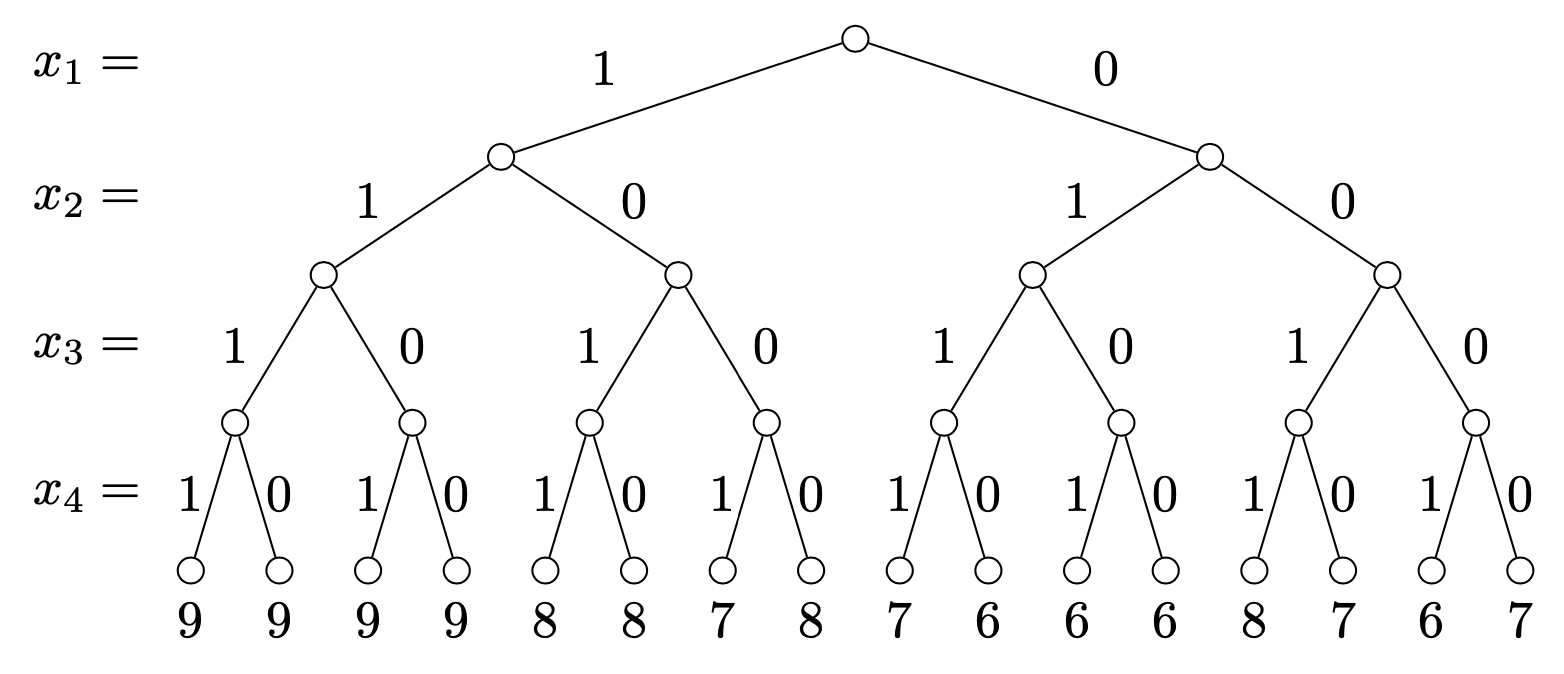
\includegraphics[width=0.55\textwidth]{SearchTree.png}
	\caption{Part (b)}
\end{figure}

\item[(c)] No, it cannot be satisfied. The maximum number of satisfied clauses is 9.


\item[(d)] Once a partial assignment is found, the idea is to check how many clauses cannot be satisfied and to cut the branches once a solution with more clauses is found. The algorithm explores the tree with a DFS strategy and obtains the first solution with $x_i = 1,~ \forall i$, for which $n$ clauses cannot be satisfied. In the first branch ($ x_1 = x_2 = x_3 = x_4 = 1$), 9 clauses are satisfied, so $n = 1$ . 
Pursuing with DFS approach, we cut branches that cannot lead to a better solution, i.e., partial assignments with at least $n$ clauses that cannot be satisfied. If a better solution is found, we update $n$ before continuing the tree exploration. 
With the first branch explored, for the partial assignment $x1 = x2 = x3 = 1$, clause $\overline{x_1} \vee  \overline{x_3}$ cannot be satisfied by any choice of the variable $x_4$, and therefore, we do not explore the branch $x_4 = 0$. Then, for the partial assignment $x_1 = x_2 = 1$, all clauses can be satisfied; we explore the branch with $x_3 = 0$, but then clause $x_3$ cannot be satisfied and we do not go further. Similarly, we stop the exploration at $x1 = 1$ and $x2 = 0$ because clause $\overline{x_1} \vee x_2$ cannot be satisfied, and then we stop at $x_1 = 0$ because clause $x1$ cannot be satisfied.

%\item[(e)] Let $t_i$ be the number of satisfied clauses when we set the values of $x_i$, and $f_i$ be the number of false clauses at the same time (all the terms of the clause must be already set to false). It is clear that the algorithm guarantees $t_i \ge f_i$.
%
%On the other hand, after the algorithms terminates, $\sum t_i$ is the total number of satisfied clauses in the formula and $\sum f_i$ is the total number of false clauses. Therefore,  $\sum t_i \geq \sum f_i$ which means at least half of the clauses are satisfied, i.e. the algorithm is $\frac{1}{2}$-approximation.
\end{itemize}
% -----------------------------------------------------------------------
\end{document}
